\section{eo\-One\-Max\-Init$<$ Genotype\-T $>$ Class Template Reference}
\label{classeo_one_max_init}\index{eoOneMaxInit@{eoOneMaxInit}}
Always write a comment in this format before class definition if you want the class to be documented by Doxygen.  


{\tt \#include $<$eo\-One\-Max\-Init.h$>$}

Inheritance diagram for eo\-One\-Max\-Init$<$ Genotype\-T $>$::\begin{figure}[H]
\begin{center}
\leavevmode
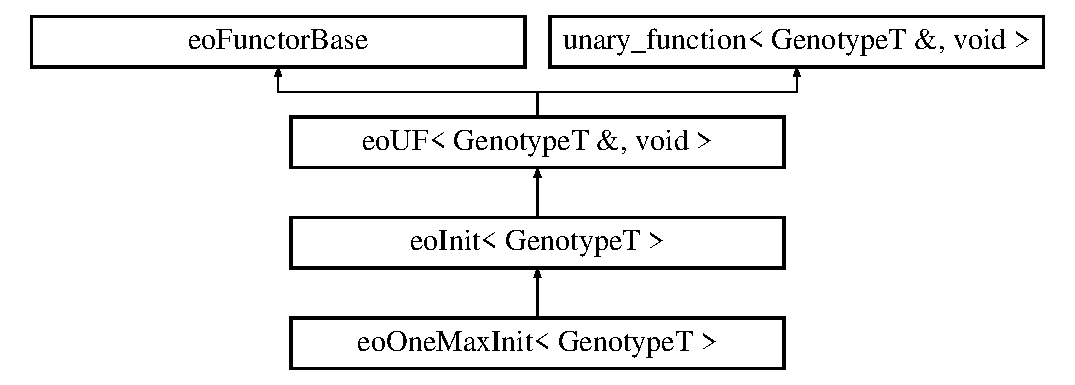
\includegraphics[height=4cm]{classeo_one_max_init}
\end{center}
\end{figure}
\subsection*{Public Member Functions}
\begin{CompactItemize}
\item 
{\bf eo\-One\-Max\-Init} (unsigned \_\-vec\-Size)\label{classeo_one_max_init_a0}

\begin{CompactList}\small\item\em Ctor - no requirement. \item\end{CompactList}\item 
void {\bf operator()} (Genotype\-T \&\_\-genotype)
\begin{CompactList}\small\item\em initialize a genotype \item\end{CompactList}\end{CompactItemize}
\subsection*{Private Attributes}
\begin{CompactItemize}
\item 
unsigned {\bf vec\-Size}\label{classeo_one_max_init_r0}

\end{CompactItemize}


\subsection{Detailed Description}
\subsubsection*{template$<$class Genotype\-T$>$ class eo\-One\-Max\-Init$<$ Genotype\-T $>$}

Always write a comment in this format before class definition if you want the class to be documented by Doxygen. 

There is NO ASSUMPTION on the class Genoype\-T. In particular, it does not need to derive from {\bf EO}{\rm (p.\,\pageref{class_e_o})} (e.g. to initialize atoms of an {\bf eo\-Vector}{\rm (p.\,\pageref{classeo_vector})} you will need an {\bf eo\-Init$<$Atom\-Type$>$}{\rm (p.\,\pageref{classeo_init})}) 



Definition at line 26 of file eo\-One\-Max\-Init.h.

\subsection{Member Function Documentation}
\index{eoOneMaxInit@{eo\-One\-Max\-Init}!operator()@{operator()}}
\index{operator()@{operator()}!eoOneMaxInit@{eo\-One\-Max\-Init}}
\subsubsection{\setlength{\rightskip}{0pt plus 5cm}template$<$class Genotype\-T$>$ void {\bf eo\-One\-Max\-Init}$<$ Genotype\-T $>$::operator() (Genotype\-T \& {\em \_\-genotype})\hspace{0.3cm}{\tt  [inline, virtual]}}\label{classeo_one_max_init_a1}


initialize a genotype 

\begin{Desc}
\item[Parameters:]
\begin{description}
\item[{\em \_\-genotype}]generally a genotype that has been default-constructed whatever it contains will be lost \end{description}
\end{Desc}


Implements {\bf eo\-UF$<$ Genotype\-T \&, void $>$} {\rm (p.\,\pageref{classeo_u_f_a1})}.

Definition at line 44 of file eo\-One\-Max\-Init.h.

References eo\-Rng::flip().

The documentation for this class was generated from the following file:\begin{CompactItemize}
\item 
eo\-One\-Max\-Init.h\end{CompactItemize}
